\documentclass[12pt,onecolumn,notitlepage]{article}
\usepackage[margin=0.5in]{geometry}
\usepackage{amsmath}
\usepackage{gensymb}
\usepackage{graphicx}
\usepackage{amsthm}
\usepackage{mathrsfs}
\usepackage{txfonts}
\usepackage{cite}
\usepackage{cases}
\usepackage{subfig}
\usepackage[breaklinks=true]{hyperref}
\usepackage{listings}
\usepackage[latin1]{inputenc}
\usepackage{color}
\usepackage{array}

\newcommand*{\comb}[2]{{}^{#1}C_{#2}}
\title{Hardware Assignment Report}
\author{Gajarla Rithika (BT22BTECH11013)}
\date{}
\begin{document}
\maketitle

\begin{LARGE}
{Random Number generation using Shift Registers}
\end{LARGE} \\

   \section*{Components required :}
\begin{enumerate}

  \setlength\itemsep{0pt} % Adjust the spacing between points
  \item  Breadboard -1   
\item Seven-segment display(common anode)-1
\item decoder(7447)-1
\item D flip-flops(7474)-2 
\item XOR gate(7486) -1   
\item 555 IC (Timer IC)-1
\item Resistor(1M$\Omega$)-1  
\item Resistor(1K$\Omega$)-1  
\item Capacitor(100nF)-1   
\item Capacitor(10nF)-1 
\item Connecting wires-20  
\end{enumerate} 

  \section*{Description of Each Component:}
\begin{itemize}
\setlength\itemsep{0pt}
\item Breadboard: A platform with interconnected sockets used for prototyping and testing electronic circuits.

\item Decoder: Decodes binary inputs from the D flip-flops and activates corresponding outputs based on the binary pattern.

\item D flip-flops: Sequential logic circuits that store and transfer a single bit of binary data. In this context, they act as part of the shift register, holding the binary values and shifting them based on the clock pulses.

\item Resistors: Passive electronic components that control the flow of electric current in a circuit. In this context, resistors may be used to provide current limiting or voltage division.

\item Capacitors: Passive components used to store and release electrical energy. In this circuit, capacitors may be used in conjunction with resistors to determine the frequency of the clock signal produced by the 555 IC.

\item Connecting wires: Used to make electrical connections between different components on the breadboard.

\item Seven-segment display: A display device that can show numerical digits and certain characters. In this circuit, it is used to display the generated random numbers.

\item XOR gate: A logic gate that outputs true (1) if the number of input signals that are true (1) is odd. In the context of the shift register, XOR gates introduce feedback loops that create randomness in the system.

\item 555 IC: A popular integrated circuit that can be configured as an astable multivibrator, producing a continuous stream of clock pulses. In this circuit, the 555 IC is used to generate the clock signal for the shift register.
\end{itemize}

\begin{figure}[h!]
  \centering
  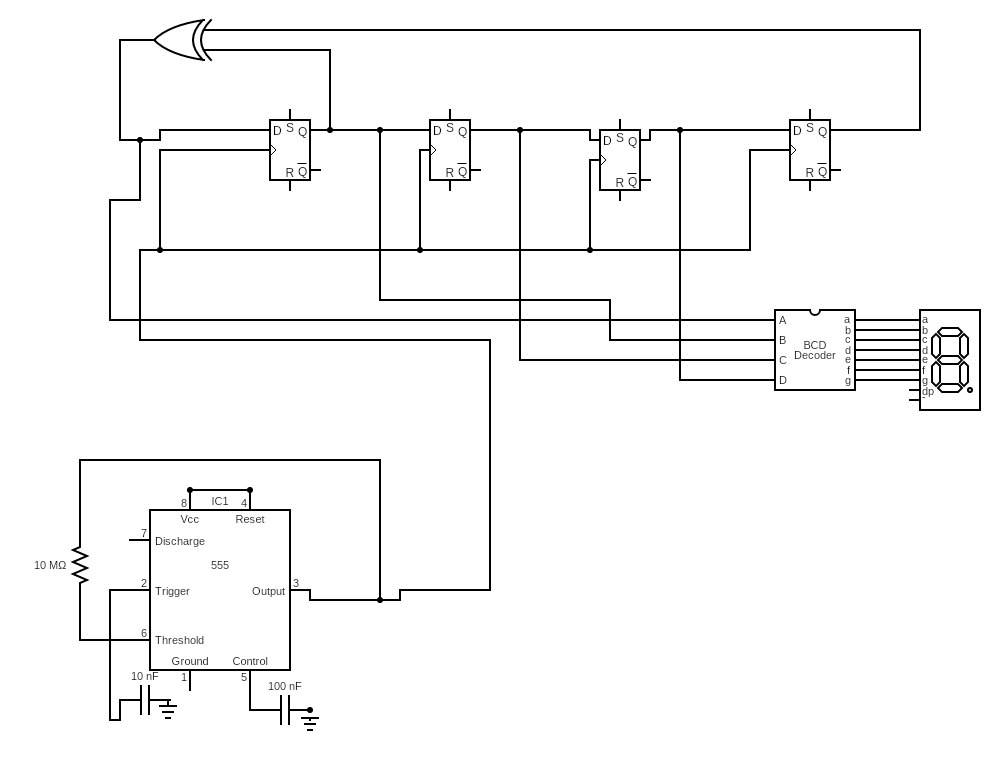
\includegraphics[width=0.5\textwidth]{blockdiag.jpg}
  \caption{Block diagram of the circuit}
  \label{fig:Circuit}
\end{figure}

\begin{figure}[h!]
  \centering
  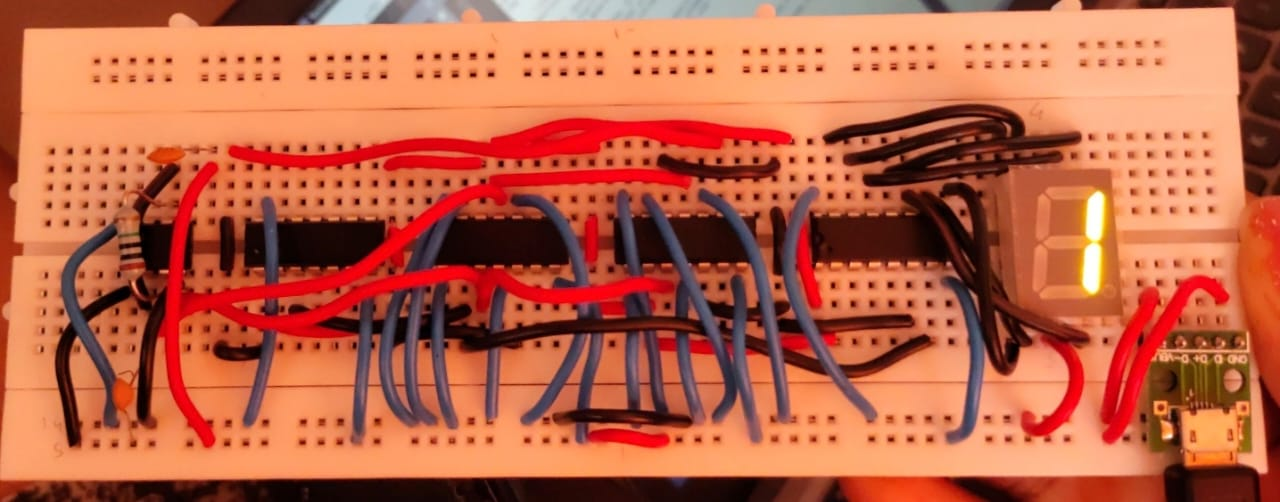
\includegraphics[width=0.5\textwidth]{circuit.jpg}
  \caption{Random Number generation using Shift registers and XOR Gate}
  \label{fig:Circuit}
\end{figure}

 
\end{document}
